\datos{color}{}{}

\subsection{\textit{FLIR Kobra 725}}

El \textit{Kobra 725}, Figura \ref{kobra725}, desarrollado por \textit{Teledyne FLIR} a partir de 2021, es un robot terrestre 
de intervención equipado con un sistema de locomoción basado en orugas de alta tracción. 
Diseñado para operaciones de desactivación de explosivos (\textit{EOD}), reconocimiento, inspección 
y rescate, destaca por su capacidad para superar obstáculos, su modularidad y su elevada 
carga útil. Su arquitectura robusta y su movilidad lo convierten en una plataforma de referencia 
en robótica táctica moderna. \\

Sus usos principales incluyen la inspección remota en entornos peligrosos, la manipulación 
de objetos mediante su brazo robotizado, la exploración de zonas colapsadas, la vigilancia 
y la intervención en escenarios de riesgo químico, biológico o explosivo. Su despliegue es 
habitual en cuerpos de seguridad y equipos de emergencia. \\

La arquitectura \textit{software} del \textit{Kobra 725} sigue un modelo centralizado, con un ordenador embarcado 
que gestiona la percepción, el control de locomoción y la supervisión del sistema. El operador 
interactúa mediante una estación de control remota que envía comandos de alto nivel y recibe 
vídeo, telemetría y datos sensoriales. El robot integra cámaras \textit{HD}, sensores térmicos, \textit{IMU} y 
módulos de comunicación cifrada, permitiendo operación segura en tiempo real. \\

El método de locomoción se basa en un sistema de orugas de alta adherencia combinado con 
\textit{flippers} articulados que permiten subir escaleras, superar escombros y ajustar la 
postura del robot para mejorar la estabilidad. Este sistema proporciona movilidad fiable en 
terrenos irregulares, superficies resbaladizas y entornos no estructurados. \\

\begin{wrapfigure}{r}{0.32\textwidth}
    \centering
    \vspace{-10pt}
    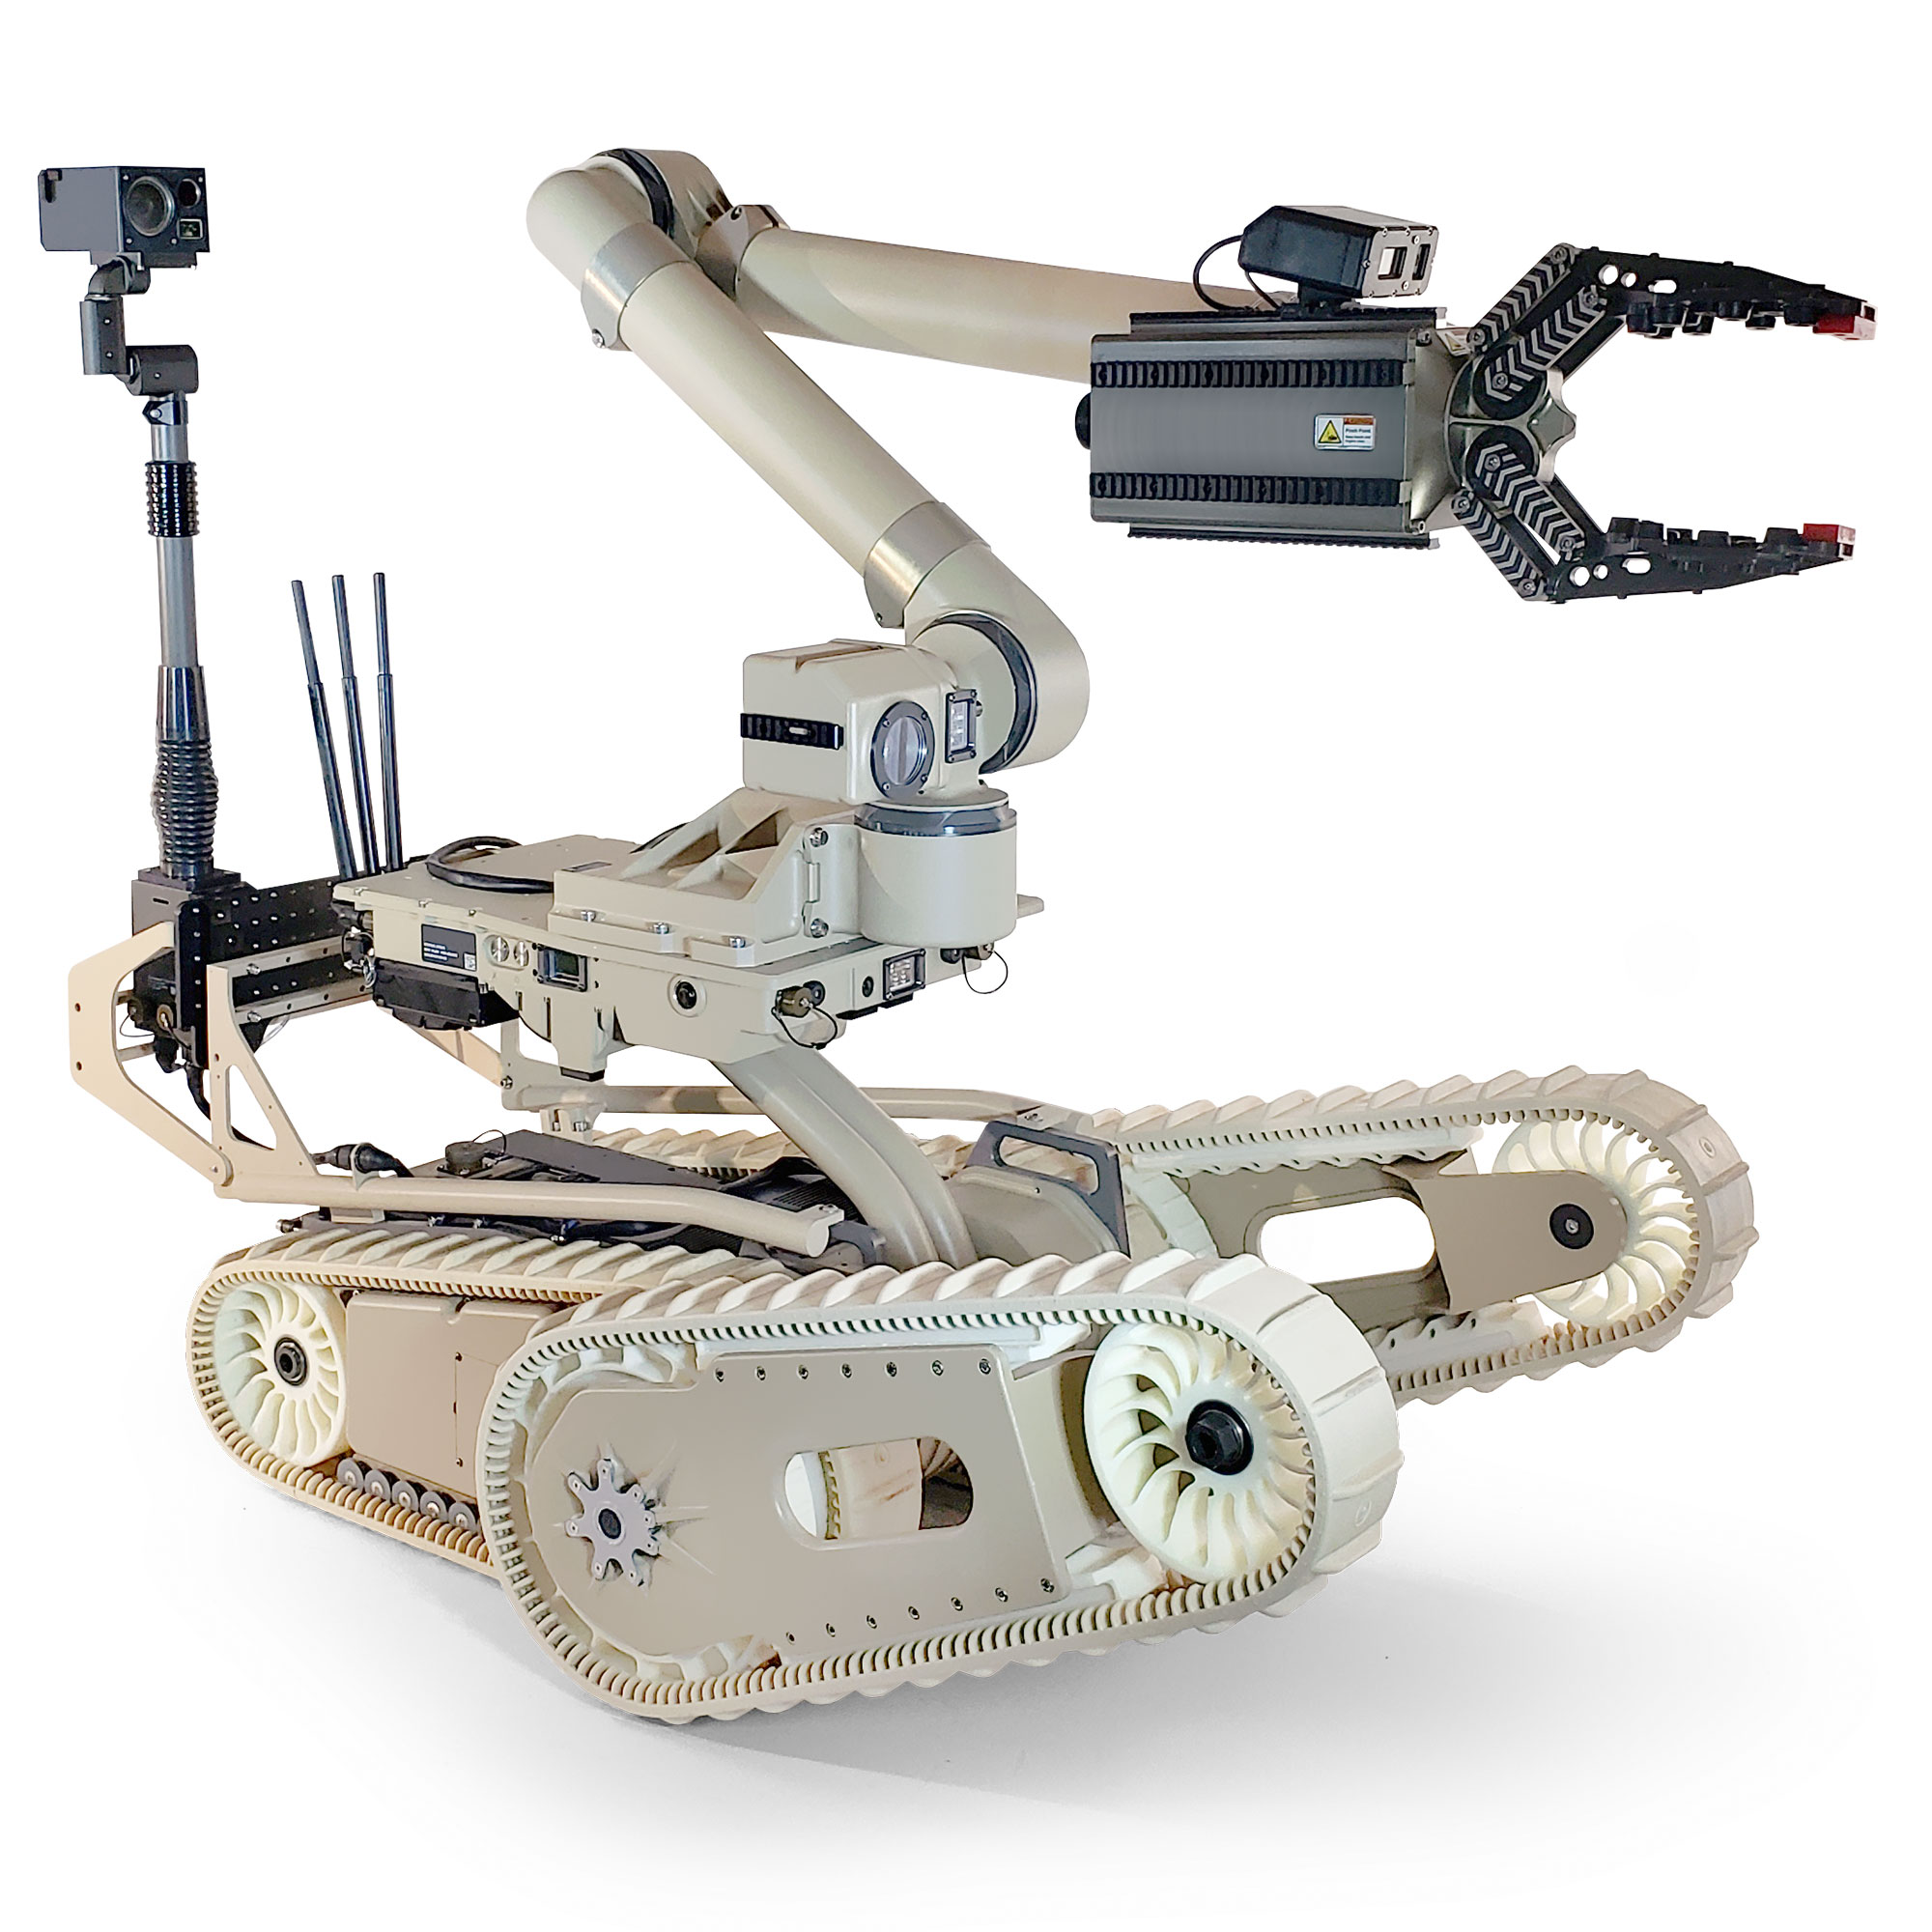
\includegraphics[width=0.28\textwidth]{Images/flirKobra725.jpg}
    \caption{\textit{FLIR Kobra 725}.}
    \label{kobra725}
    \vspace{-10pt}
\end{wrapfigure}

\subsection*{Referencias}

\cite{Kobra725Ref} \fullcite{Kobra725Ref}.
